\vspace{-2.5mm}
\subsection{Equivariant Operations for Irreps Features}
\vspace{-2.5mm}
\label{subsec:equivariant_operations}

%As irreps features encode directional and equivariant information in channel dimensions without complicating graph structures, we can adopt irreps features and inherit the design of existing networks through utilizing equivariant operations.
\revision{We discuss below equivariant operations, which serve as building blocks for equivariant graph attention and other modules, and analyze how they remain equivariant in Sec.~\ref{appendix:subsec:equivariant_operations}.}
%They include the equivariant version of the original operations in Transformers and the depth-wise tensor product, as illustrated in Fig.~\ref{fig:equivariant_operation} in appendix. %, an efficient version of tensor product.
They include the equivariant version of operations in Transformers and depth-wise tensor products as shown in Fig.~\ref{fig:equivariant_operation}. % in appendix. %, an efficient version of tensor product.

%\note{(We describe the difference of the operations in Equiformer from what has already introduced in Background.)}

%Since the internal representations are E(3) features, we replace the original operations with equivariant counterparts to preserve E(3)-equivariance and discuss equivariant versions of operations used in Transformer.
%Besides, we adopt the operation of tensor product to exchange the information contained in different type-$l$ vectors.

%\todo{Add figure for each of them!}

\vspace{-2.5mm}
\paragraph{Linear.}
Linear layers are generalized to irreps features by transforming different type-$L$ vectors separately.
Specifically, we apply separate linear operations to each group of type-$L$ vectors.
We remove bias terms for non-scalar features with $L > 0$ as biases do not depend on inputs, and therefore, including biases for type-$L$ vectors with $L > 0$ can break equivariance.
%Note that linear layers can be regarded as a special case of tensor product between E(3) features and type-$0$ constant one.

\vspace{-2.5mm}
\paragraph{Layer Normalization.}
Transformers adopt layer normalization (LN)~\citep{layer_norm} to stabilize training.
%\revision{
%Given input $x \in \mathbb{R}^{N \times C}$, with $N$ being the number of nodes and $C$ the number of channels, LN  calculates the linear transformation of normalized input as follows:
Given input $x \in \mathbb{R}^{N \times C}$, with $N$ being the number of nodes and $C$ the number of channels, LN  calculates the linear transformation of normalized input as $\text{LN}(x) = \left( \frac{  x - \mu_{C}  }{\sigma_{C}} \right) \circ \gamma + \beta$,
%\begin{equation}
%\text{LN}(x) = \frac{x - \mu_{C}}{\sigma_{C}} \circ \gamma + \beta
%\end{equation}
where $\mu_{C}, \sigma_{C} \in \mathbb{R}^{N \times 1}$ are mean and standard deviation of input $x$ along the channel dimension, $\gamma, \beta \in \mathbb{R}^{1 \times C}$ are learnable parameters, and $\circ$ denotes element-wise product.
%}
By viewing standard deviation as the root mean square value (RMS) of L2-norm of type-$L$ vectors, LN can be generalized to irreps features.
Specifically, given input $x \in \mathbb{R}^{N \times C \times (2L + 1)}$ of type-$L$ vectors, the output is
$\text{LN}(x) = \left( \frac{x}{\text{RMS}_{C}(\text{norm}(x))} \right) \circ \gamma$,
%\begin{equation}
%\text{LN}(x) = \frac{x}{\text{RMS}_{C}(\text{norm}(x))} \circ \gamma
%\end{equation}
where $\text{norm}(x) \in \mathbb{R}^{N \times C \times 1}$ calculates the L2-norm of each type-$L$ vectors in $x$, and $\text{RMS}_{C}(\text{norm}(x)) \in \mathbb{R}^{N \times 1 \times 1}$ calculates the RMS of L2-norm with mean taken along the channel dimension.
%%%We remove mean and biases for type-$L$ vectors with $L \neq 0$ following linear layers.
We remove means and biases for type-$L$ vectors with $L \neq 0$.

\vspace{-2.5mm}
\paragraph{Gate.}
We use the gate activation~\citep{3dsteerable} for equivariant activation function as shown in Fig.~\ref{fig:equivariant_operation}(c).
Typical activation functions are applied to type-$0$ vectors.
For vectors of higher $L$, we multiply them with non-linearly transformed type-$0$ vectors for equivariance.
Specifically, given input $x$ containing non-scalar $C_{L}$ type-$L$ vectors with $ 0 < L \leq L_{max}$ and $(C_0 + \sum_{L=1}^{L_{max}} C_L)$ type-$0$ vectors, we apply SiLU~\citep{silu, swish} to the first $C_0$ type-$0$ vectors and sigmoid function to the other $\sum_{L=1}^{L_{max}} C_L$ type-$0$ vectors to obtain non-linear weights and multiply each type-$L$ vector with corresponding non-linear weights.
After the gate activation, the number of channels for type-$0$ vectors is reduced to $C_0$.

\vspace{-2.5mm}
\paragraph{Depth-wise Tensor Product.}
The tensor product defines interaction between vectors of different $L$.
%%%To improve its efficiency, we use the depth-wise tensor product (DTP), which restricts one type-$L$ vector in output irreps features depends only on one type-$L'$ vector in input irreps features, where $L$ can be equal to or different from $L'$.
To improve its efficiency, we use the depth-wise tensor product (DTP), where one type-$L$ vector in output irreps features depends only on one type-$L'$ vector in input irreps features as illustrated in Fig.~\ref{fig:equivariant_operation}(d) and Fig.~\ref{fig:depthwise_tensor_product_e3nn}, with $L$ being equal to or different from $L'$.
This is similar to depth-wise convolution~\citep{mobilenet}, where one output channel depends on only one input channel. 
%, and therefore, we call it depth-wise tensor product (DTP).
Weights $w$ in the DTP can be input-independent or conditioned on relative distances, and the DTP between two tensors $x$ and $y$ is denoted as $x \otimes_{w}^{DTP} y$. % $x \tens_{w}^{DTP} y$.
%\todo{(Mention tensor product weights in Background)}
Note that the one-to-one dependence of channels can significantly reduce the number of weights and thus memory complexity when weights are conditioned on relative distances.
In contrast, if one output channel depends on all input channels, in our case, this can lead to out-of-memory errors when weights are parametrized by relative distances.

\begin{figure*}[t]
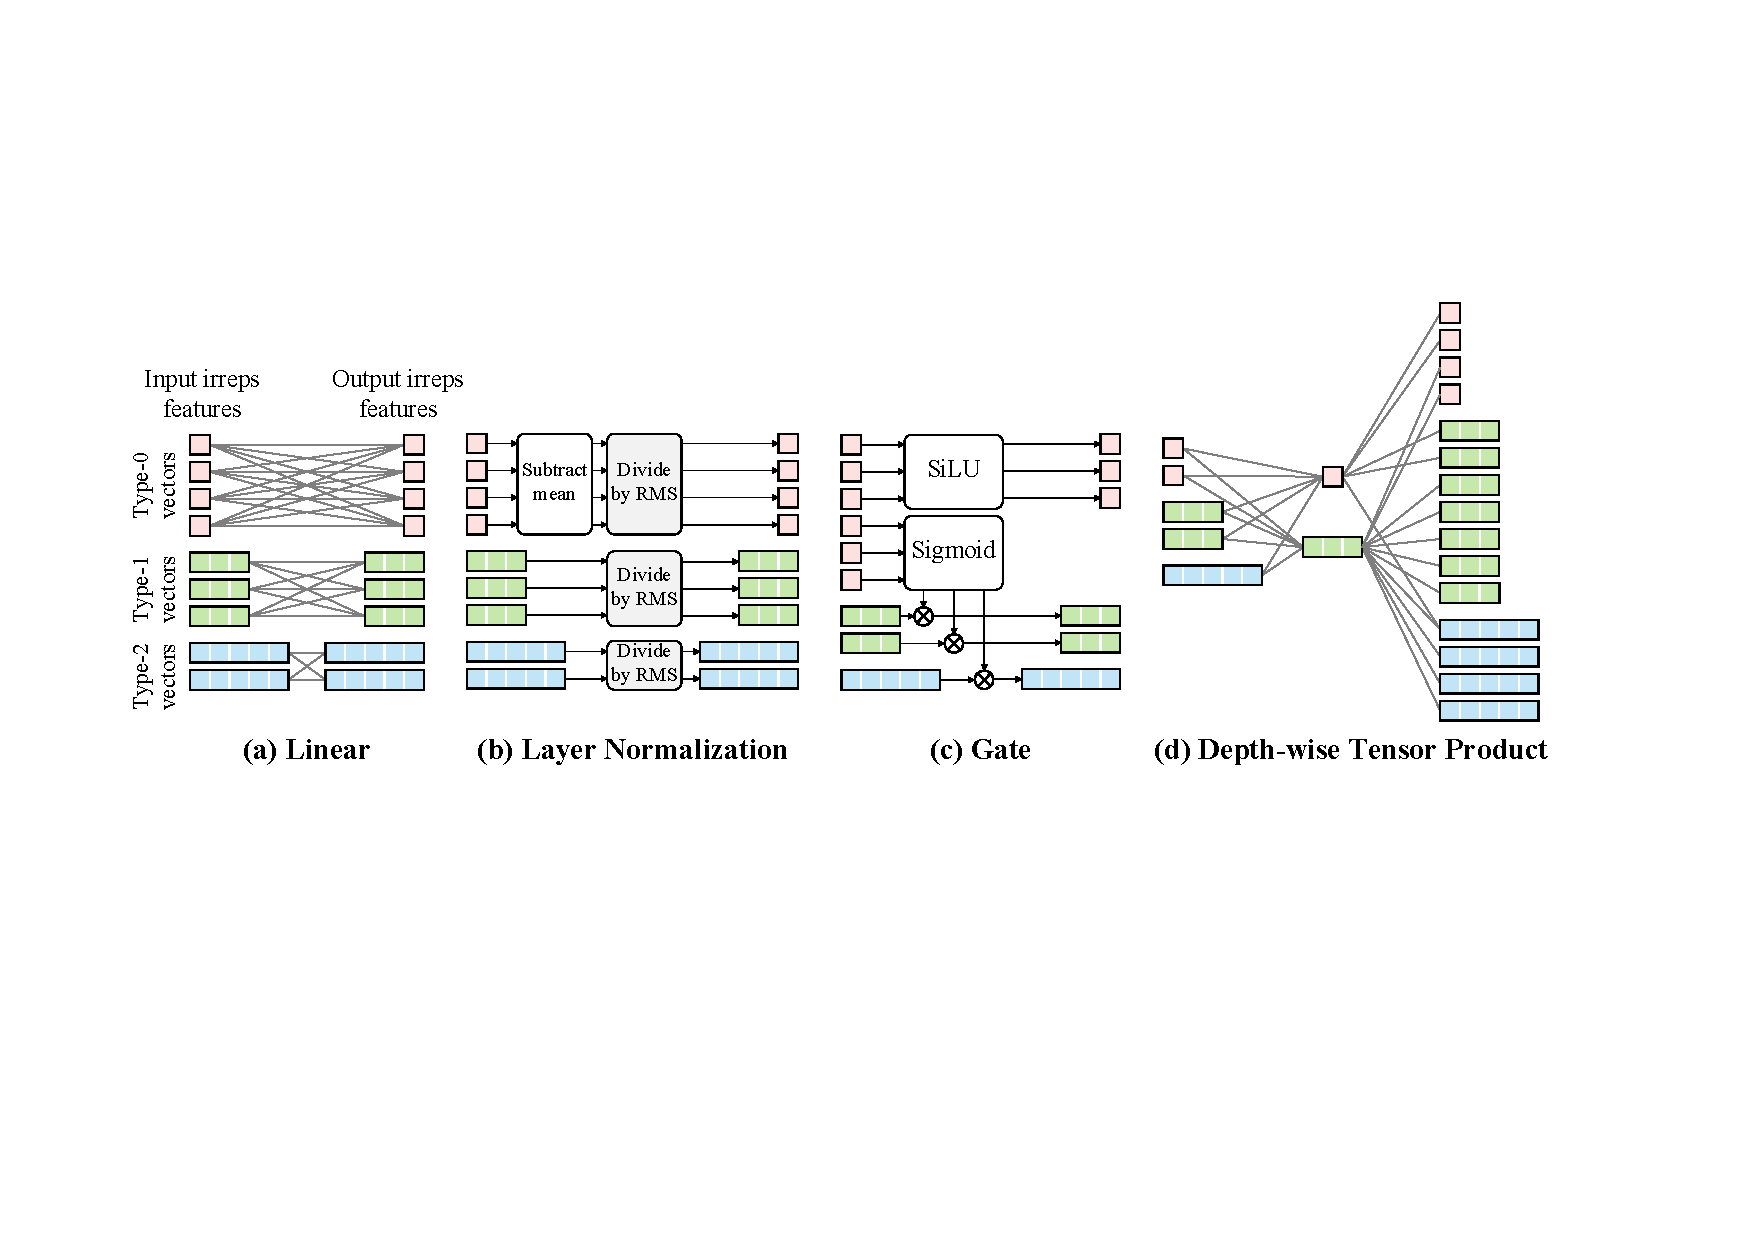
\includegraphics[width=0.85\linewidth]{figure/equivariant_operation.pdf}
\centering
\vspace{-3.5mm}
\caption{
\textbf{Equivariant operations used in Equiformer.}
%For ``Linear'', each gray line has one learnable weight.
\textbf{(a)} Each gray line between input and output irreps features contains one learnable weight.
%Note that the number of output channels can be different from that of input channels.
%The number of output channels can be different from that of input channels.
%For ``Layer Normalization'', ``RMS'' denotes root mean squared value with mean taken along channel dimension, and we remove multiplying by $\gamma$ in this figure for simplicity.  
%\textbf{(b)} ``RMS'' denotes the root mean square value (RMS) along the channel dimension.
\textbf{(b)} ``RMS'' denotes the root mean square value along the channel dimension.
For simplicity, we have removed multiplying by $\gamma$ here.
\textbf{(c)} Gate layers are equivariant activation functions where non-linearly transformed scalars are used to gate non-scalar irreps features.
\textbf{(d)} The left two irreps features correspond to two input irreps features, and the rightmost one is the output irreps feature.
%For ``Depth-wise Tensor Product'', the left two irreps features correspond to two input irreps features, and the rightmost one is output irreps feature.
The two gray lines connecting two vectors in the input irreps features and one vector in the output irreps feature form a path and contain one learnable weight.
An alternative visualization of depth-wise tensor products can be found in Fig.~\ref{fig:depthwise_tensor_product_e3nn} in appendix.
We show $SE(3)$-equivariant operations here, which can be generalized to $E(3)$-equivariant features.
}

\vspace{-4mm}
\label{fig:equivariant_operation}
\end{figure*}
